%!TEX root = ../Thesis.tex
\lstset {language=C++}

\chapter{VRInteractions}
\label{ch:vrinteractions}
\lhead{\emph{VRInteractions}}
In dit hoofdstuk worden de keuzes voor en de werking van de VRInteractions \gls{ue4} plugin besproken. 
Voor elk component in de plugin wordt de werking en mogelijkheden getoond. Daarnaast wordt voor elk component, waar relevant, besproken hoe de workshops de design keuzes beïnvloed heeft.

\section{De plugin}
De VRInteractions plugin is een combinatie van C++ code, Blueprints en overschrijfbare game modes.
De plugin heeft als doel om de \gls{vr} specifieke logica te verbergen voor gameplay logica zodat niet-programmeurs interactieve \gls{vr} omgevingen kunnen maken.

De plugin is ontwikkeld met de workflow die beschreven wordt in paragraaf ~\ref{ch:workflow}.

De plugin bevat op moment van schrijven de volgende componenten:
\begin{itemize}
	\item Gamemodes
		\begin{itemize}
			\item VRInteractionsFlyTroughGameMode
			\item VRInteractionsGameMode
		\end{itemize}
	\item Characters
		\begin{itemize}
			\item VRInteractionBaseCharacter
			\item VRInteractionCharacter
			\item VRInteractionsFlyCharacter
		\end{itemize}
	\item VRInteractionsPlayerController
	\item VRInteractionsCameraManager
	\item VRInteractionsHud
	\item LookEventsComponent
	\item CircleMenu
	\item VRMovableMesh
\end{itemize}

\section{Gamemodes}
De plugin bevat de gamemodes VRInteractionsFlyTroughGameMode en VRInteractionsGameMode. Deze modes zijn beide een uitbreiding van de voorbeeld \gls{ue4} characters. Beide gamemodes zijn geschikt voor zowel de Oculus als de GearVR. 

De gamemodes zijn bedoelt om de basis instellingen voor \gls{vr} in te stellen en zijn voor de meeste applicaties voldoende. In het geval dat er iets in de gamemode aangepast moet worden is het mogelijk de instelling te overschrijven of de gehele gamemode over te erven.

Omdat er gebruik wordt gemaakt van een aantal input events is het aan te raden om een project altijd te beginnen als First Person Template.

\subsection{VRInteractionsGameMode}
De VRInteractionsGameMode maakt gebruik van de VRInteractionCharacter, VRInteractionsHud, VRInteractionsPlayerController en de VRInteractionsCameraManager. 

De gamemode is bedoeld voor spellen waarin de speler kan rondlopen en zorgt ervoor dat de headset juist wordt geïnstalleerd en de juiste controllers ingesteld staan.

\subsection{VRInteractionsFlyTroughGameMode}
De VRInteractionsFlyTroughGameMode is een gestripte versie van de VRInteractionsGameMode en maakt gebruik van de VRInteractionsFlyCharacter, VRInteractionsHud, VRInteractionsPlayerController en VRInteractionsCameraManager.

Deze gamemode is bedoelt voor VR projecten waarin de speler met behulp van Matinee rondvliegt.

\section{Characters}
De VRInteractionsCharacters bevatten alle beweging- en camera instellingen zoals ooghoogte. De instellingen zijn gebaseerd op de \gls{vr} guidelines van Epic\footnote{\href{https://docs.unrealengine.com/latest/INT/Platforms/VR/ContentSetup/index.html}{https://docs.unrealengine.com/latest/INT/Platforms/VR/ContentSetup/index.html} }.


\subsection{VRInteractionBaseCharacter}
De VRInteractionBaseCharacter is de basis voor de VRInteractionCharacter en de VRInteractionsFlyCharacter. Deze characters bevatten de instellingen voor de camera hoogte en enkele \gls{vr} gerelateerde logica zoals het roteren van de speler op basis van zijn kijkrichting.

Ook wordt hierin de GearVR touch pad input afgehandeld.

Het is niet de bedoeling deze classe direct te implementeren. In plaats daarvan kan er gekozen worden voor de VRInteractionCharacter of de VRInteractionsFlyCharacter. Als er een nieuw soort character gemaakt moet worden kan die natuurlijk overerven van de VRInteractionBaseCharacter.

\subsection{VRInteractionCharacter}
De VRInteractionCharacter is bedoelt voor spellen waarin de speler rond kan lopen. De instellingen en functies zijn op basis van de \gls{ue4} \gls{vr} guidelines en de testen van de \gls{vr} demo gemaakt.

\subsection{VRInteractionsFlyCharacter}
De VRInteractionCharacter is bedoelt voor spellen waarin de speler op een rails loopt. Het is mogelijk deze character makkelijk in Matinee te gebruiken. Verschil met de VRInteractionCharacter, naast het niet registeren van controle gerelateerde input, is dat de camera niet op ooghoogte maar in het midden van de character geplaatst wordt. Dit maakt het maken van de Matinee sequences logischer.

\section{VRInteractionsPlayerController}
De VRInteractionsPlayerController is gebaseerd op de standaard PlayerController van Epic. De controller is verantwoordelijk voor het correct doorgeven van de input naar de ingestelde Character.

In de controller zorgen wij ook dat de rotatie van de controller klopt met de rotatie van de headset op het moment dat de headset aangezet wordt, zo kan de headset tijdens het spelen aan en uit gezet worden.

\section{VRInteractionsCameraManager}
De VRInteractionsCameraManager is gebaseerd op de standaard VRInteractionsCameraManager van Epic. Deze Manager is verantwoordelijk voor het instellen van camera instellingen zoals de FOV. 

\section{VRInteractionsHud}
De VRInteractionsHud is de basis \gls{hud} die een cirkel tekent in het midden van het scherm om aan te geven dat er naar een actor met een LookEvent gekeken wordt.

\begin{figure}[H]
  \centering
    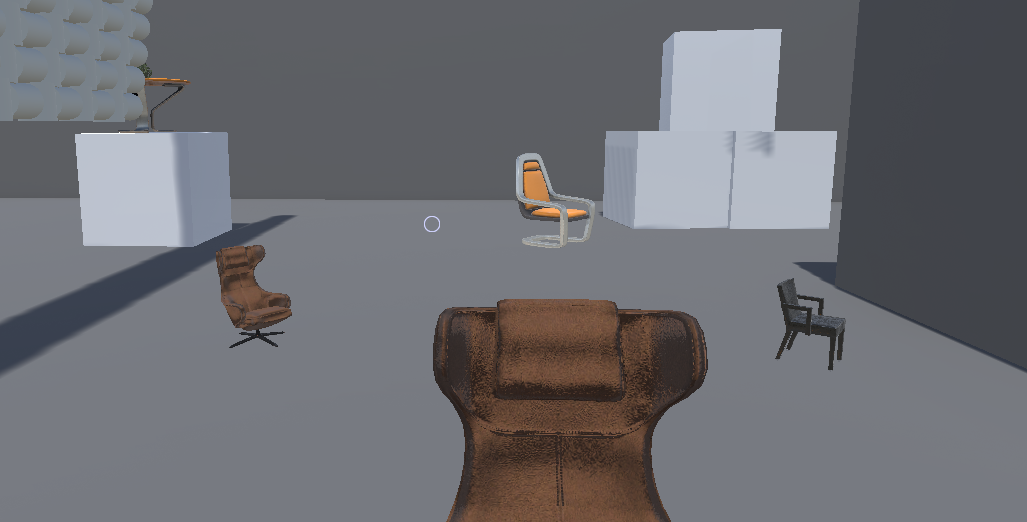
\includegraphics[width=\linewidth,height=\textheight,keepaspectratio]{HudExample}
    \caption{De cirkel die getekend wordt op het moment dat er naar een Actor met een LookEventsComponent gekeken wordt.}
\end{figure}

De \gls{hud} is afhankelijk van de VRInteractionsDataSingleton. Om te zorgen dat deze altijd correct wordt ingeladen kan de singleton als Game Singleton Class ingesteld worden. De singleton wordt namelijk gebruikt om informatie van de LookEventsComponents te verzamelen.

\section{LookEventsComponent}
De LookEventsComponent vuurt events af op het moment dat er naar de opgegeven trigger gekeken word. Het is mogelijk om meerdere LookEventsComponents aan dezelfde actor toe te voegen waardoor onder andere menu's op basis van kijken gemaakt kunnen worden.

De LookEventsComponent is de basis van de plugin en bijna alle nadere componenten zijn hierop gebaseerd. 

\subsection{Implementatie}
Voor een aantal weken zijn de LookEvents als zowel een Actor als een Component geïmplementeerd. Het voordeel van een Actor implementatie is dat er vanuit world editor in het rechter muisknop menu event's gekoppeld kunnen worden.

\begin{figure}[!ht]
  \centering
    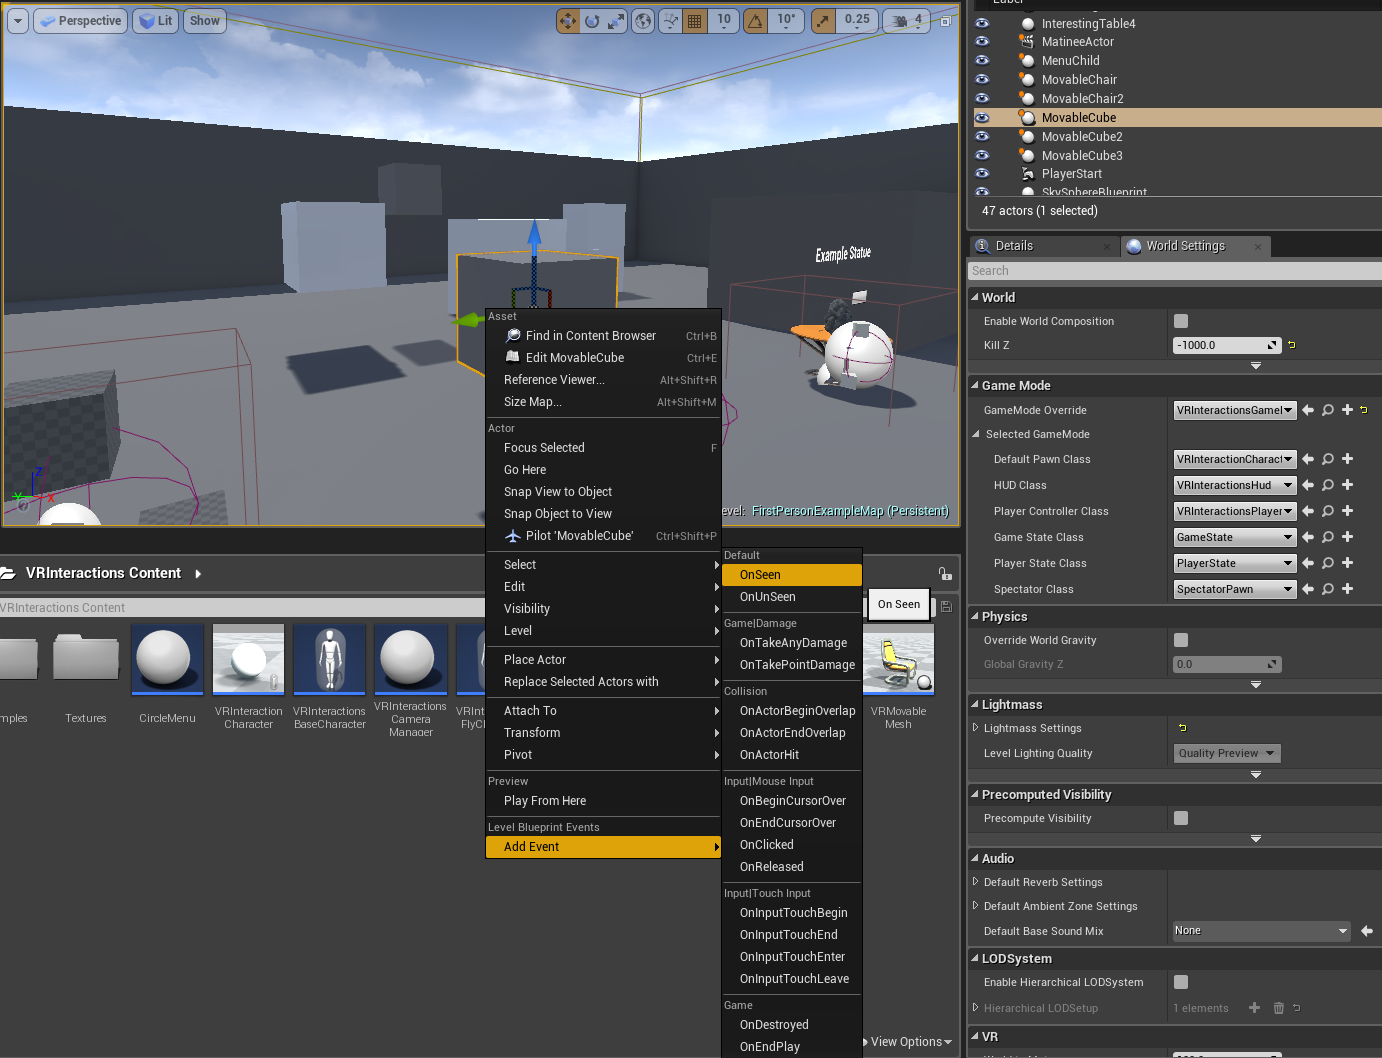
\includegraphics[width=\linewidth,height=\textheight,keepaspectratio]{VRInteractions_OnSeenLevel}
    \caption{Voorbeeld van het kopellen van een event aan een actor.}
\end{figure}

Dit heeft als nadeel dat het event direct in het level Blueprint gekoppeld wordt wat aanmoedigt om hier de logica te plaatsen terwijl dit vaak in een Blueprint Actor zou moeten gebeuren.

Ook is het lastig de Actor implementatie binnen een Blueprint Actor te gebruiken, dit kan via een ActorComponent. Het ActorComponent maakt het niet mogelijk om instellingen via de editor te doen en verplicht daardoor om alle settings via Blueprints te zetten, wat omslachtig en fout gevoelig is.

Daarom is er voor de Component implementatie gekozen. Dit maakt het makkelijk om via de Blueprint editor events toe te voegen en kunnen er meerdere LookEvents gebruikt worden. Het is nog steeds mogelijk om een level Blueprint event binnen de actor te maken die gekoppeld is aan het event van de component.

\subsection{Events}
De koppeling met Blueprints zit zich voornamelijk in de events die afgevuurd worden door de LookEventsComponent. Dit is ook de interface waarmee de niet-programmeurs de interactie kunnen programmeren.

Er kan op twee manieren logica aan een event gekoppeld worden. De eerste is via het component menu zoals getoond in figuur~\ref{fig:ComponentMenuEvent} en de tweede zoals getoond in figuur~\ref{fig:ComponentReferenceAsign}.

\begin{figure}[H]
  \centering
    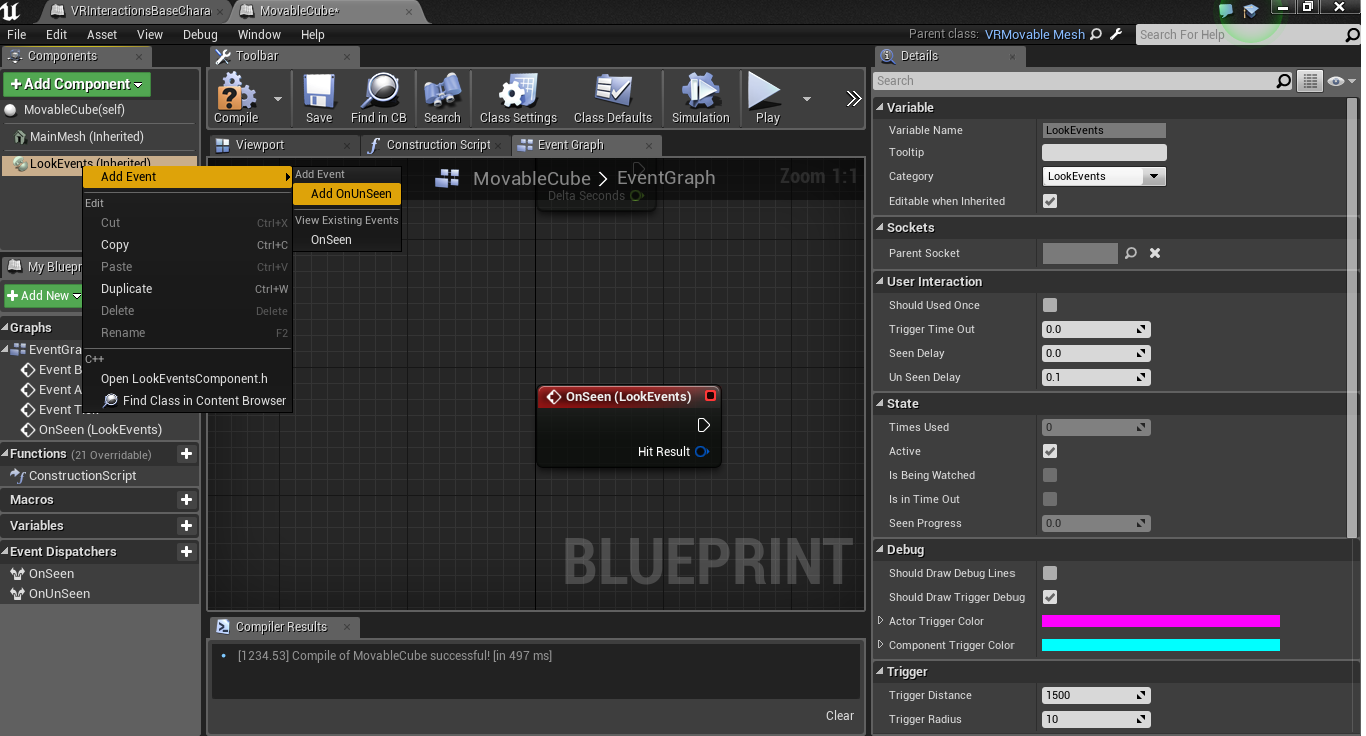
\includegraphics[width=\linewidth,height=\textheight,keepaspectratio]{VRInteractions_EventComponent}
    \caption{Voorbeeld van het koppelen van een event via het component menu.}
    \label{fig:ComponentMenuEvent}
\end{figure}

\begin{figure}[H]
  \centering
    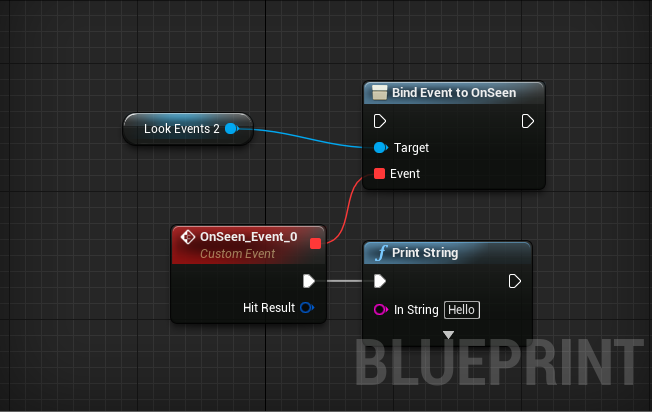
\includegraphics[width=\linewidth,height=\textheight,keepaspectratio]{VRInteractions_OnSeenAsign}
    \caption{Voorbeeld van het koppelen van een event via een reference naar een LookEventsComponent}
    \label{fig:ComponentReferenceAsign}
\end{figure}

Vooral de eerste manier werd als duidelijk ervaren voor de niet-programmeurs terwijl voor manier twee wel uitleg nodig was, in de tweede workshop bijlage~\ref{appendix:workshop2}.

\subsection{Instelling}
De volgende instellingen zijn mogelijk voor de LookEventsComponent:

\begin{itemize}
	\item bShouldUsedOnce
	\item TimesUsed
	\item TriggerTimeOut
	\item SeenDelay
	\item UnSeenDelay
	\item bShouldDrawDebugLines
	\item bShouldDrawTriggerDebug
	\item ActorTriggerColor
	\item ComponentTriggerColor
	\item TriggerDistance
	\item TriggerRadius
	\item bActive
	\item SeenTrigger
	\item UnSeenTrigger
\end{itemize}

\subsubsection{Seen en UnSeen trigger}
De trigger is het object waar naar gekeken kan worden. Er kan voor zowel het triggeren van het Seen event als voor het triggeren van het UnSeen event een ander object gekozen worden.

Er is hier voor gekozen nadat het duidelijk werd dat er vaak een animatie plaats vind of er extra objecten, bijvoorbeeld een menu, tevoorschijn komen die niet in de originele trigger passen.

\begin{figure}[!ht]
  \centering
    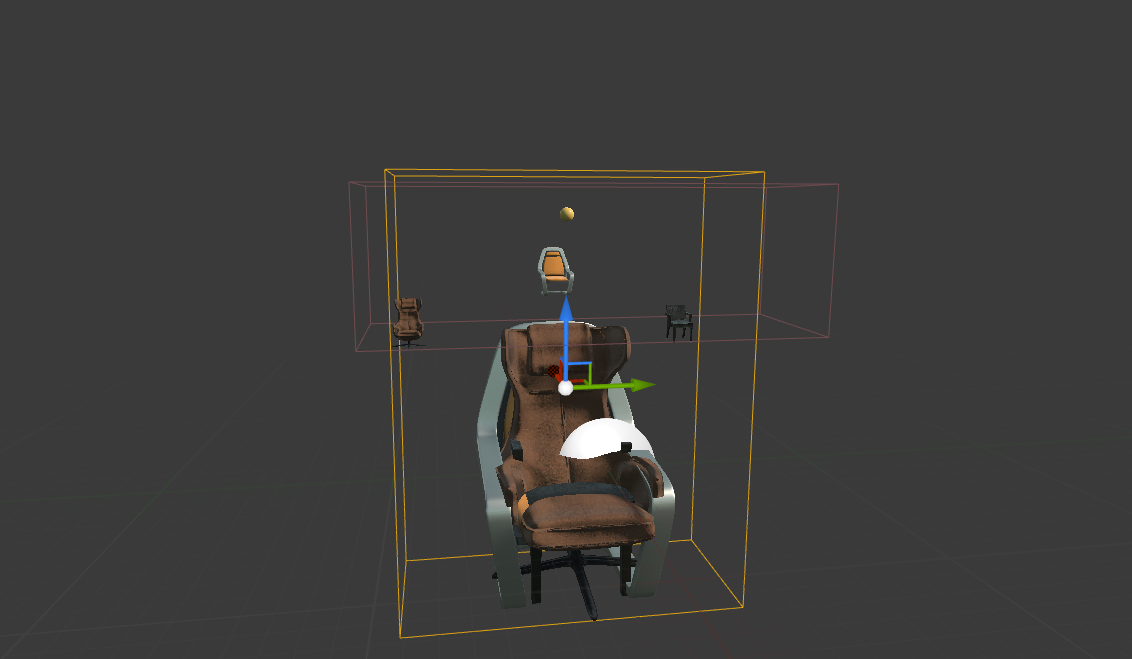
\includegraphics[width=\linewidth,height=\textheight,keepaspectratio]{Voorbeeld_SeenUnseenTriggerBox}
    \caption{Een voorbeeld waarin de geselecteerde trigger box het menu toont en het menu getoond blijft zolang er naar de tweede trigger box gekeken word}
\end{figure}

Als er niet specifiek een trigger opgegeven word word de Actor die het component bevat als Seen en Unseen trigger gezien. De triggers kunnen via blueprint gezet worden.

\begin{figure}[!ht]
  \centering
    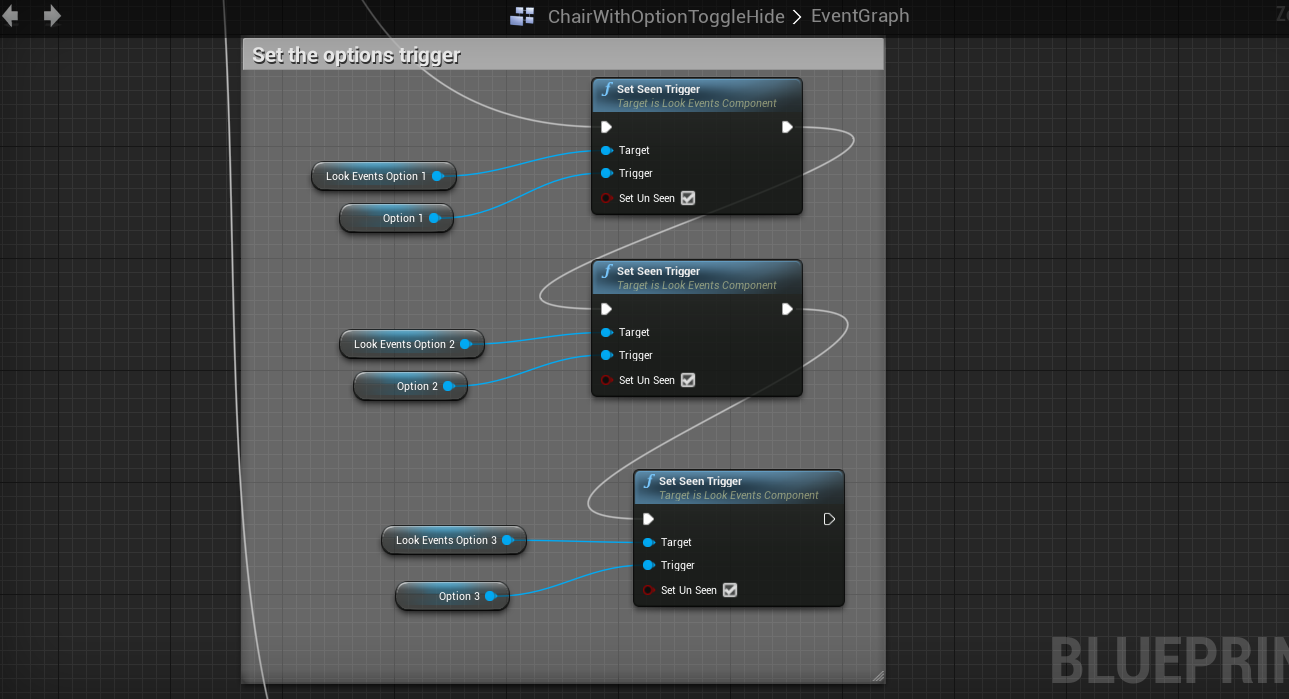
\includegraphics[width=\linewidth,height=\textheight,keepaspectratio]{SetSeenTriggerExample}
    \caption{Een voorbeeld van het instellen van de triggers voor drie verschillende LookEventComponents}
\end{figure}

\subsection{Debugging}
Tijdens de workshops werd er aangegeven dat het lastig was om de LookEvents te debuggen omdat de triggers niet te zien zijn. Er is voor gekozen om dezelfde debugging voor raytraces te implementeren voor de LookEvents.

\begin{figure}[!ht]
  \centering
    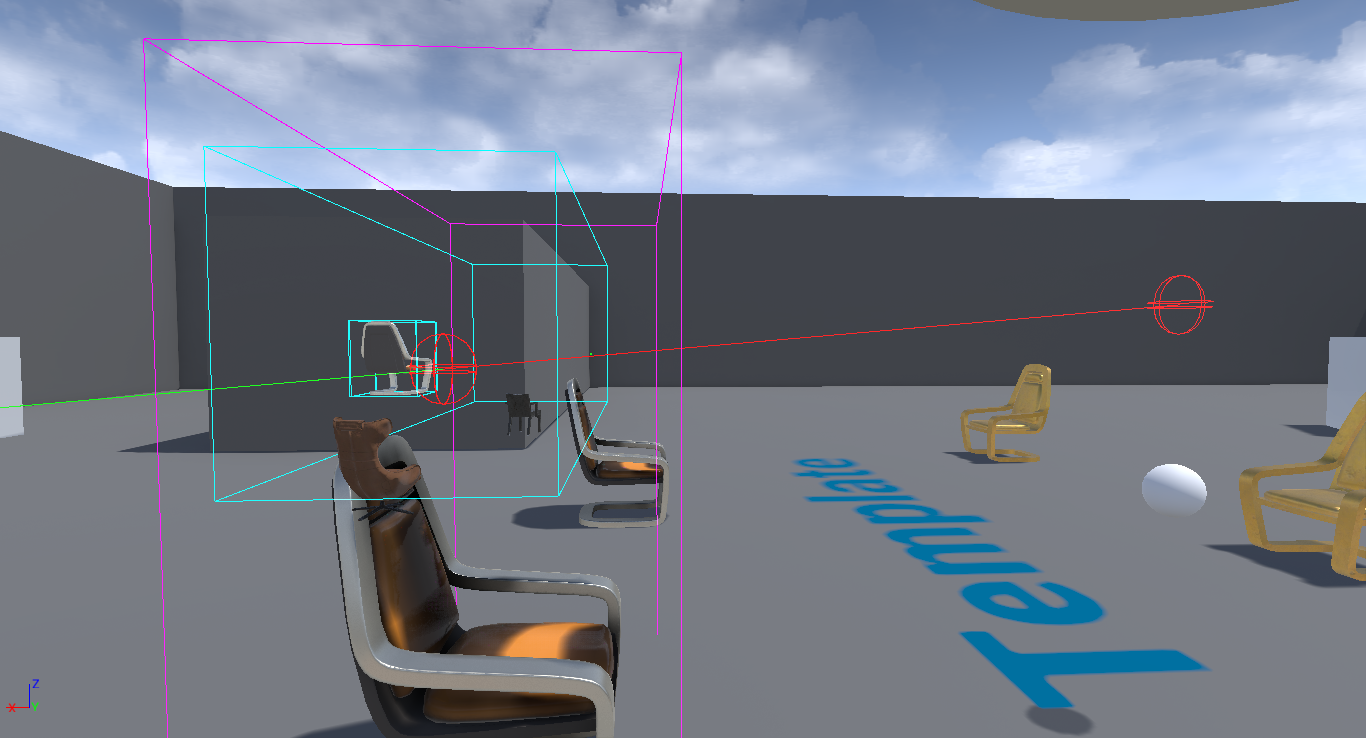
\includegraphics[width=\linewidth,height=\textheight,keepaspectratio]{debugInformatieVanLookEvents}
    \caption{Voorbeeld van debug informatie die een LookEvent kan tekenen.}
\end{figure}

Er wordt een lijn getekend vanaf de speler ter lengte van de TriggerDistance. Vervolgens word er een vierkant getekend rond de active triggers, er kan een kleur voor Actors en voor Components opgegeven worden. Als er een blocking hit is, door een niet doorzichtig object, word er een cirkel getekend met als diameter de TriggerRadius op de plek waar de blocking hit plaats vond.

\section{CircleMenu}
Het CircleMenu genereert een menu van LookEventsComponents op basis van een lijst van meshes.

\begin{figure}[!ht]
  \centering
    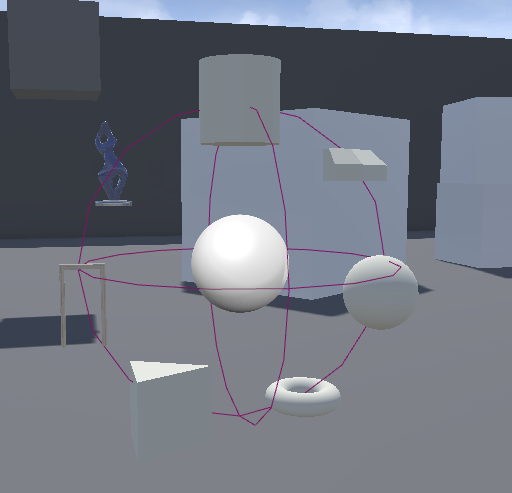
\includegraphics[width=\linewidth/2,height=\textheight/2,keepaspectratio]{CircleMenu_voorbeeld}
    \caption{Voorbeeld van het CircleMenu.}
\end{figure}

\begin{figure}[!ht]
  \centering
    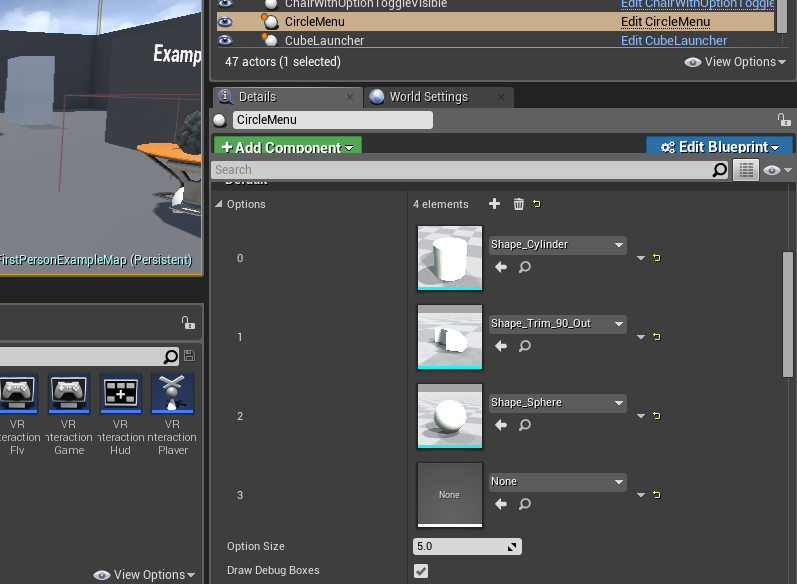
\includegraphics[width=\linewidth/2,height=\textheight/2,keepaspectratio]{CircleMenu_AddMesh}
    \caption{Het instellen van de opties in een CircleMenu.}
\end{figure}

Om te zorgen dat de meshes correct gepositioneerd worden in een cirkel kan er een grootte van de meshes opgegeven worden en worden de meshes op basis hiervan individueel gescaled. Ook wordt er rekening mee gehouden dat het pivot point van een mesh zich niet altijd in het midden bevindt en wordt er berekend wat het midden van de mesh is om vervolgens de mesh correct te positioneren. Er is ook een optie om het menu altijd richting de speler te tonen. 

\begin{figure}[!ht]
  \centering
    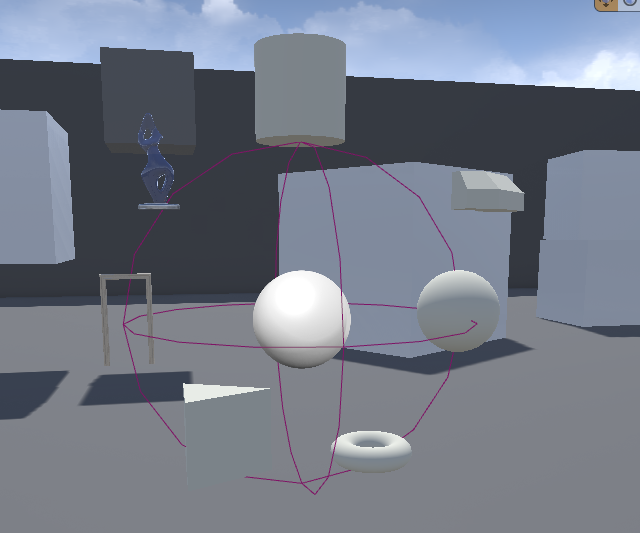
\includegraphics[width=\linewidth/2,height=\textheight/2,keepaspectratio]{CircleMenu_NotCorrectedExample}
    \caption{Het CIrcleMenu zonder dat de pivot gecorrigeerd word.}
\end{figure}

De combinatie van het genereren en volgen van de speler zorgt ervoor dat de niet-programmeurs uitgebreide menu's in \gls{vr} kunnen creëren.

\subsection{Instellingen}
\begin{itemize}
	\item Options
	\item OptionsSize
	\item DrawDebugBoxes
	\item TriggerDistance
	\item FollowPlayer
\end{itemize}

\subsection{Events}
Voor het circlemenu moest een Actor gemaakt worden, omdat components geen subcomponents kunnen hebben. Dit maakt het mogelijk om via het rechtermuisknop menu events te koppelen in het level Blueprint.

\begin{figure}[!ht]
  \centering
    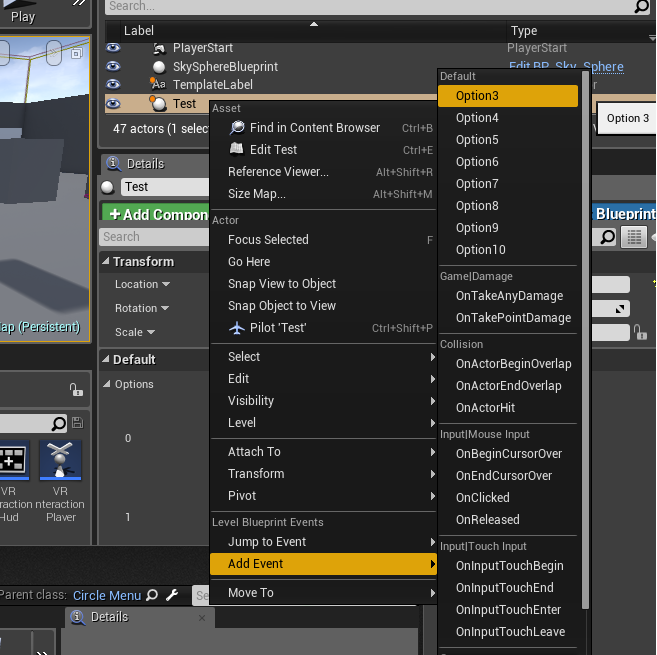
\includegraphics[width=\linewidth/2,height=\textheight/2,keepaspectratio]{CircleMenu_AddEventLevel}
    \caption{Het koppelen van een event via het level Blueprint.}
\end{figure}

Helaas maakt dit het gebruik van het CircleMenu in een Actor omslachtig. Er moet namelijk gebruik gemaakt worden van een ChildActor component. De ChildActor component maakt het niet mogelijk om instellingen via het detail menu in te stellen. Hierdoor zal het daadwerkelijk CircleMenu via Blueprints benaderd moeten worden.

\begin{figure}[H]
  \centering
    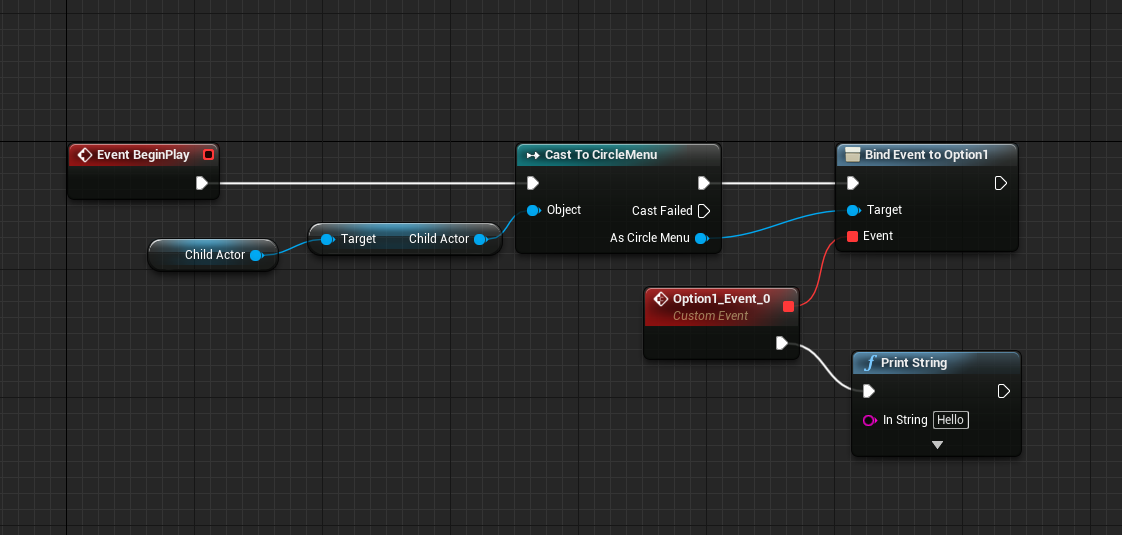
\includegraphics[width=\linewidth,height=\textheight,keepaspectratio]{CircleMenu_EventInActor}
    \caption{Het koppelen van het instellen van een event in een CircleMenu als ChildActor component.}
\end{figure}

Deze omslachtigere manier van event koppeling vergt beter kennis van Blueprints en werd als onduidelijk ervaren door de niet-programmeurs.

\section{VRMovableMesh}
De VRMovableMesh is een Actor die verplaatsbaar is door middel van een interactie knop en het kijken naar de bestemming. Het object wordt versleept naar de locatie waar naar gekeken wordt zolang men een knop indrukt.

\begin{figure}[!ht]
  \centering
  	\begin{subfigure}[b]{\linewidth/3}
    	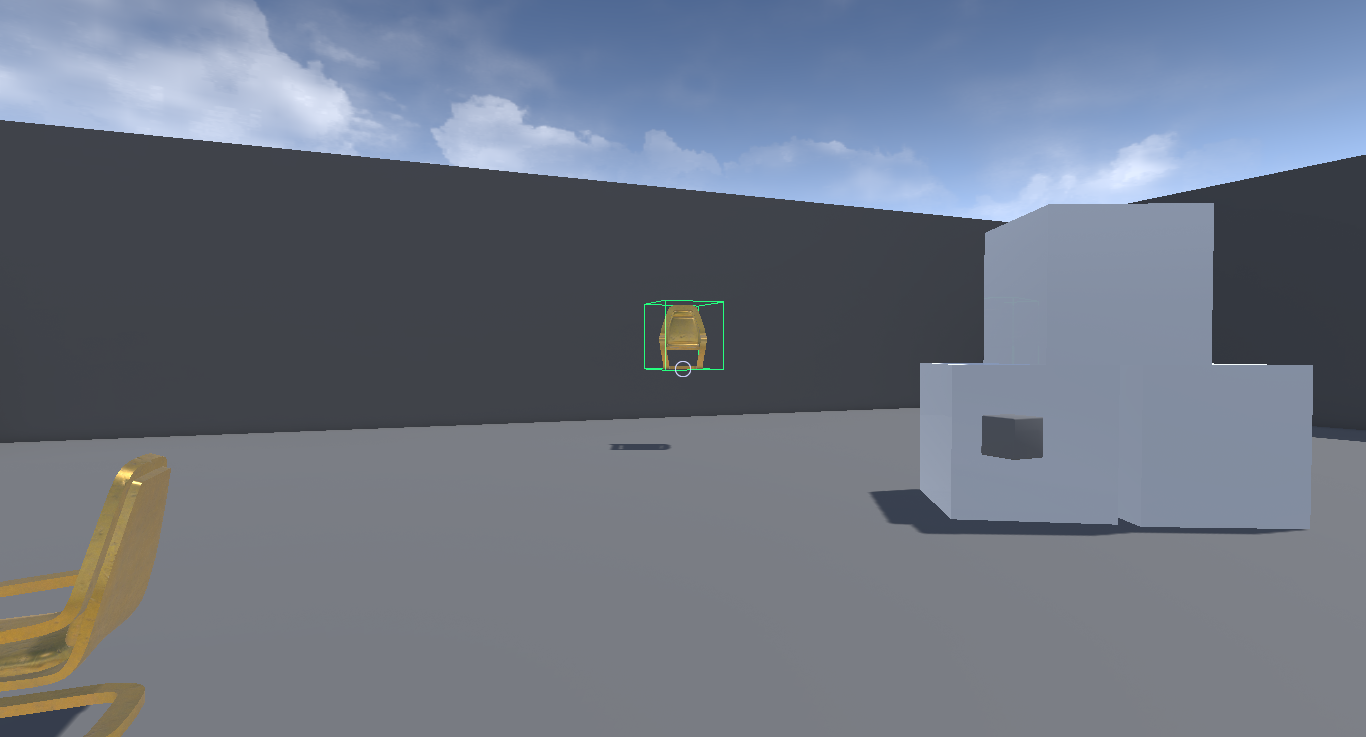
\includegraphics[width=60mm]{MovableMesh_place1}
    	\label{fig:a}
	\end{subfigure}

	\begin{subfigure}[b]{\linewidth/3}
    	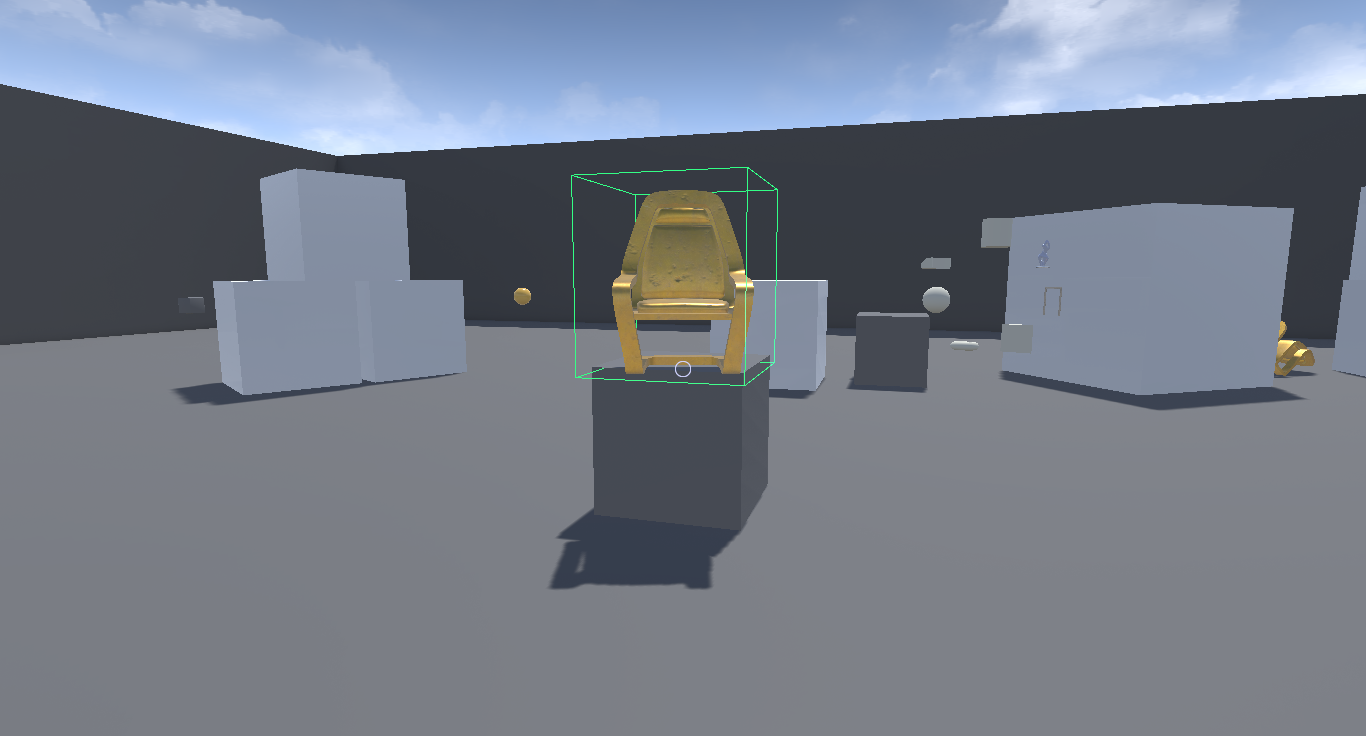
\includegraphics[width=60mm]{MovableMesh_place2}
    	\label{fig:b}
	\end{subfigure}

	\caption{Voorbeeld van het verplaatsen van een MovableMesh.}
\end{figure}

\subsection{Instellingen}

\begin{itemize}
	\item MainMesh
	\item MaxDistance
	\item MinDistance
	\item Throwable
	\item bSetRotation
	\item bIsInteracting
\end{itemize}